% Options for packages loaded elsewhere
\PassOptionsToPackage{unicode}{hyperref}
\PassOptionsToPackage{hyphens}{url}
%
\documentclass[
]{article}
\usepackage{amsmath,amssymb}
\usepackage{iftex}
\ifPDFTeX
  \usepackage[T1]{fontenc}
  \usepackage[utf8]{inputenc}
  \usepackage{textcomp} % provide euro and other symbols
\else % if luatex or xetex
  \usepackage{unicode-math} % this also loads fontspec
  \defaultfontfeatures{Scale=MatchLowercase}
  \defaultfontfeatures[\rmfamily]{Ligatures=TeX,Scale=1}
\fi
\usepackage{lmodern}
\ifPDFTeX\else
  % xetex/luatex font selection
\fi
% Use upquote if available, for straight quotes in verbatim environments
\IfFileExists{upquote.sty}{\usepackage{upquote}}{}
\IfFileExists{microtype.sty}{% use microtype if available
  \usepackage[]{microtype}
  \UseMicrotypeSet[protrusion]{basicmath} % disable protrusion for tt fonts
}{}
\makeatletter
\@ifundefined{KOMAClassName}{% if non-KOMA class
  \IfFileExists{parskip.sty}{%
    \usepackage{parskip}
  }{% else
    \setlength{\parindent}{0pt}
    \setlength{\parskip}{6pt plus 2pt minus 1pt}}
}{% if KOMA class
  \KOMAoptions{parskip=half}}
\makeatother
\usepackage{xcolor}
\usepackage[margin=1in]{geometry}
\usepackage{color}
\usepackage{fancyvrb}
\newcommand{\VerbBar}{|}
\newcommand{\VERB}{\Verb[commandchars=\\\{\}]}
\DefineVerbatimEnvironment{Highlighting}{Verbatim}{commandchars=\\\{\}}
% Add ',fontsize=\small' for more characters per line
\newenvironment{Shaded}{}{}
\newcommand{\AlertTok}[1]{\textcolor[rgb]{1.00,0.00,0.00}{\textbf{#1}}}
\newcommand{\AnnotationTok}[1]{\textcolor[rgb]{0.38,0.63,0.69}{\textbf{\textit{#1}}}}
\newcommand{\AttributeTok}[1]{\textcolor[rgb]{0.49,0.56,0.16}{#1}}
\newcommand{\BaseNTok}[1]{\textcolor[rgb]{0.25,0.63,0.44}{#1}}
\newcommand{\BuiltInTok}[1]{\textcolor[rgb]{0.00,0.50,0.00}{#1}}
\newcommand{\CharTok}[1]{\textcolor[rgb]{0.25,0.44,0.63}{#1}}
\newcommand{\CommentTok}[1]{\textcolor[rgb]{0.38,0.63,0.69}{\textit{#1}}}
\newcommand{\CommentVarTok}[1]{\textcolor[rgb]{0.38,0.63,0.69}{\textbf{\textit{#1}}}}
\newcommand{\ConstantTok}[1]{\textcolor[rgb]{0.53,0.00,0.00}{#1}}
\newcommand{\ControlFlowTok}[1]{\textcolor[rgb]{0.00,0.44,0.13}{\textbf{#1}}}
\newcommand{\DataTypeTok}[1]{\textcolor[rgb]{0.56,0.13,0.00}{#1}}
\newcommand{\DecValTok}[1]{\textcolor[rgb]{0.25,0.63,0.44}{#1}}
\newcommand{\DocumentationTok}[1]{\textcolor[rgb]{0.73,0.13,0.13}{\textit{#1}}}
\newcommand{\ErrorTok}[1]{\textcolor[rgb]{1.00,0.00,0.00}{\textbf{#1}}}
\newcommand{\ExtensionTok}[1]{#1}
\newcommand{\FloatTok}[1]{\textcolor[rgb]{0.25,0.63,0.44}{#1}}
\newcommand{\FunctionTok}[1]{\textcolor[rgb]{0.02,0.16,0.49}{#1}}
\newcommand{\ImportTok}[1]{\textcolor[rgb]{0.00,0.50,0.00}{\textbf{#1}}}
\newcommand{\InformationTok}[1]{\textcolor[rgb]{0.38,0.63,0.69}{\textbf{\textit{#1}}}}
\newcommand{\KeywordTok}[1]{\textcolor[rgb]{0.00,0.44,0.13}{\textbf{#1}}}
\newcommand{\NormalTok}[1]{#1}
\newcommand{\OperatorTok}[1]{\textcolor[rgb]{0.40,0.40,0.40}{#1}}
\newcommand{\OtherTok}[1]{\textcolor[rgb]{0.00,0.44,0.13}{#1}}
\newcommand{\PreprocessorTok}[1]{\textcolor[rgb]{0.74,0.48,0.00}{#1}}
\newcommand{\RegionMarkerTok}[1]{#1}
\newcommand{\SpecialCharTok}[1]{\textcolor[rgb]{0.25,0.44,0.63}{#1}}
\newcommand{\SpecialStringTok}[1]{\textcolor[rgb]{0.73,0.40,0.53}{#1}}
\newcommand{\StringTok}[1]{\textcolor[rgb]{0.25,0.44,0.63}{#1}}
\newcommand{\VariableTok}[1]{\textcolor[rgb]{0.10,0.09,0.49}{#1}}
\newcommand{\VerbatimStringTok}[1]{\textcolor[rgb]{0.25,0.44,0.63}{#1}}
\newcommand{\WarningTok}[1]{\textcolor[rgb]{0.38,0.63,0.69}{\textbf{\textit{#1}}}}
\usepackage{graphicx}
\makeatletter
\def\maxwidth{\ifdim\Gin@nat@width>\linewidth\linewidth\else\Gin@nat@width\fi}
\def\maxheight{\ifdim\Gin@nat@height>\textheight\textheight\else\Gin@nat@height\fi}
\makeatother
% Scale images if necessary, so that they will not overflow the page
% margins by default, and it is still possible to overwrite the defaults
% using explicit options in \includegraphics[width, height, ...]{}
\setkeys{Gin}{width=\maxwidth,height=\maxheight,keepaspectratio}
% Set default figure placement to htbp
\makeatletter
\def\fps@figure{htbp}
\makeatother
\setlength{\emergencystretch}{3em} % prevent overfull lines
\providecommand{\tightlist}{%
  \setlength{\itemsep}{0pt}\setlength{\parskip}{0pt}}
\setcounter{secnumdepth}{-\maxdimen} % remove section numbering
\usepackage{fontspec}
\setmainfont{NanumGothic}
\ifLuaTeX
  \usepackage{selnolig}  % disable illegal ligatures
\fi
\usepackage{bookmark}
\IfFileExists{xurl.sty}{\usepackage{xurl}}{} % add URL line breaks if available
\urlstyle{same}
\hypersetup{
  pdftitle={JTBC 1702},
  hidelinks,
  pdfcreator={LaTeX via pandoc}}

\title{JTBC 1702}
\author{}
\date{\vspace{-2.5em}}

\begin{document}
\maketitle

\subsection{Problem}\label{problem}

JTBC 뉴스룸에서는 다음과 같은 도표의 후보지지도 여론조사 결과를 보도.

\begin{Shaded}
\begin{Highlighting}[]
\NormalTok{knitr}\SpecialCharTok{::}\FunctionTok{include\_graphics}\NormalTok{(}\StringTok{"../pics/poll\_2017\_JTBC.jpg"}\NormalTok{)}
\end{Highlighting}
\end{Shaded}

\begin{center}\includegraphics[width=0.67\linewidth]{../pics/poll_2017_JTBC} \end{center}

막대의 높이에 의구심을 표한 시청자들의 항의에 직면함.

제대로 된 막대그래프를 그리면서 R Base plot과 ggplot에 대하여 학습.

\subsection{Data Setup}\label{data-setup}

\begin{Shaded}
\begin{Highlighting}[]
\FunctionTok{library}\NormalTok{(extrafont)}
\NormalTok{candidates }\OtherTok{\textless{}{-}} \FunctionTok{c}\NormalTok{(}\StringTok{"문재인"}\NormalTok{, }\StringTok{"안희정"}\NormalTok{, }\StringTok{"황교안"}\NormalTok{, }\StringTok{"안철수"}\NormalTok{, }\StringTok{"이재명"}\NormalTok{, }\StringTok{"유승민"}\NormalTok{) }
\NormalTok{rates }\OtherTok{\textless{}{-}} \FunctionTok{c}\NormalTok{(}\DecValTok{33}\NormalTok{, }\DecValTok{22}\NormalTok{, }\DecValTok{9}\NormalTok{, }\DecValTok{9}\NormalTok{, }\DecValTok{5}\NormalTok{, }\DecValTok{2}\NormalTok{)}
\NormalTok{party }\OtherTok{\textless{}{-}} \FunctionTok{c}\NormalTok{(}\StringTok{"더불어민주당"}\NormalTok{, }\StringTok{"자유한국당"}\NormalTok{, }\StringTok{"국민의당"}\NormalTok{, }\StringTok{"바른정당"}\NormalTok{)}
\NormalTok{colour\_party }\OtherTok{\textless{}{-}} \FunctionTok{c}\NormalTok{(}\StringTok{"skyblue"}\NormalTok{, }\StringTok{"lightgrey"}\NormalTok{, }\StringTok{"darkgreen"}\NormalTok{, }\StringTok{"darkblue"}\NormalTok{)}
\NormalTok{candidates\_party }\OtherTok{\textless{}{-}}  \FunctionTok{c}\NormalTok{(}\StringTok{"더불어민주당"}\NormalTok{, }\StringTok{"더불어민주당"}\NormalTok{, }\StringTok{"자유한국당"}\NormalTok{, }
                       \StringTok{"국민의당"}\NormalTok{, }\StringTok{"더불어민주당"}\NormalTok{, }\StringTok{"바른정당"}\NormalTok{)}
\FunctionTok{match}\NormalTok{(candidates\_party, party)}
\end{Highlighting}
\end{Shaded}

\begin{verbatim}
## [1] 1 1 2 3 1 4
\end{verbatim}

\begin{Shaded}
\begin{Highlighting}[]
\NormalTok{candidates\_colour }\OtherTok{\textless{}{-}}\NormalTok{ colour\_party[}\FunctionTok{match}\NormalTok{(candidates\_party, party)]}
\end{Highlighting}
\end{Shaded}

\subsection{Barplot (R Base)}\label{barplot-r-base}

\begin{Shaded}
\begin{Highlighting}[]
\FunctionTok{barplot}\NormalTok{(rates)}
\end{Highlighting}
\end{Shaded}

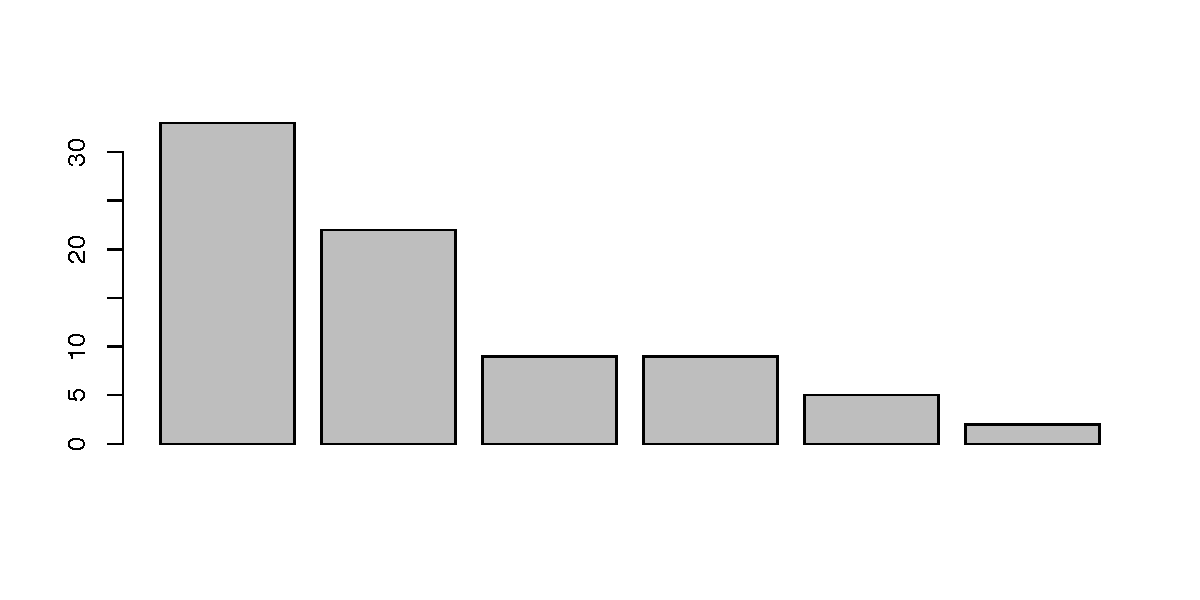
\includegraphics{poll_JTBC_1702_pdf_files/figure-latex/unnamed-chunk-2-1.pdf}

\begin{Shaded}
\begin{Highlighting}[]
\FunctionTok{library}\NormalTok{(showtext)}
\CommentTok{\# font\_add(family = "noto", regular = "/Users/kwlee/Library/Fonts/NotoSansKR{-}VariableFont\_wght.ttf")}
\CommentTok{\# showtext\_auto()}
\FunctionTok{font\_add}\NormalTok{(}\AttributeTok{family =} \StringTok{"Apple"}\NormalTok{, }\AttributeTok{regular =} \StringTok{"/System/Library/Fonts/AppleSDGothicNeo.ttc"}\NormalTok{)}
\FunctionTok{showtext\_auto}\NormalTok{()}
\FunctionTok{par}\NormalTok{(}\AttributeTok{family =} \StringTok{"Apple"}\NormalTok{)}
\NormalTok{b1 }\OtherTok{\textless{}{-}} \FunctionTok{barplot}\NormalTok{(rates, }
              \AttributeTok{axes =} \ConstantTok{FALSE}\NormalTok{, }
              \AttributeTok{col =}\NormalTok{ candidates\_colour, }
              \AttributeTok{names.arg =} \ConstantTok{NULL}\NormalTok{,}
              \AttributeTok{cex.names =} \FloatTok{1.5}\NormalTok{)}
\FunctionTok{mtext}\NormalTok{(}\AttributeTok{side =} \DecValTok{1}\NormalTok{, }\AttributeTok{at =}\NormalTok{ b1, }\AttributeTok{line =} \FloatTok{0.5}\NormalTok{, }\AttributeTok{text =}\NormalTok{ candidates, }\AttributeTok{cex =} \FloatTok{1.5}\NormalTok{)}
\FunctionTok{text}\NormalTok{(}\AttributeTok{x =}\NormalTok{ b1, }\AttributeTok{y =}\NormalTok{ rates }\SpecialCharTok{+} \FunctionTok{c}\NormalTok{(}\FunctionTok{rep}\NormalTok{(}\SpecialCharTok{{-}}\DecValTok{3}\NormalTok{, }\DecValTok{4}\NormalTok{), }\FunctionTok{rep}\NormalTok{(}\FloatTok{1.5}\NormalTok{, }\DecValTok{2}\NormalTok{)), }
     \AttributeTok{labels =}\NormalTok{ rates, }
     \AttributeTok{col =} \FunctionTok{c}\NormalTok{(}\StringTok{"black"}\NormalTok{, }\StringTok{"black"}\NormalTok{, }\StringTok{"black"}\NormalTok{, }\StringTok{"white"}\NormalTok{, }\StringTok{"black"}\NormalTok{, }\StringTok{"black"}\NormalTok{),}
     \AttributeTok{cex =} \FloatTok{1.5}\NormalTok{)}
\NormalTok{main\_title }\OtherTok{\textless{}{-}} \StringTok{"차기 대선주자 지지율(\%)"}
\FunctionTok{title}\NormalTok{(}\AttributeTok{main =}\NormalTok{ main\_title, }
      \AttributeTok{cex.main =} \DecValTok{2}\NormalTok{)}
\FunctionTok{box}\NormalTok{(}\AttributeTok{which =} \StringTok{"figure"}\NormalTok{, }\AttributeTok{lwd =} \DecValTok{3}\NormalTok{)}
\end{Highlighting}
\end{Shaded}

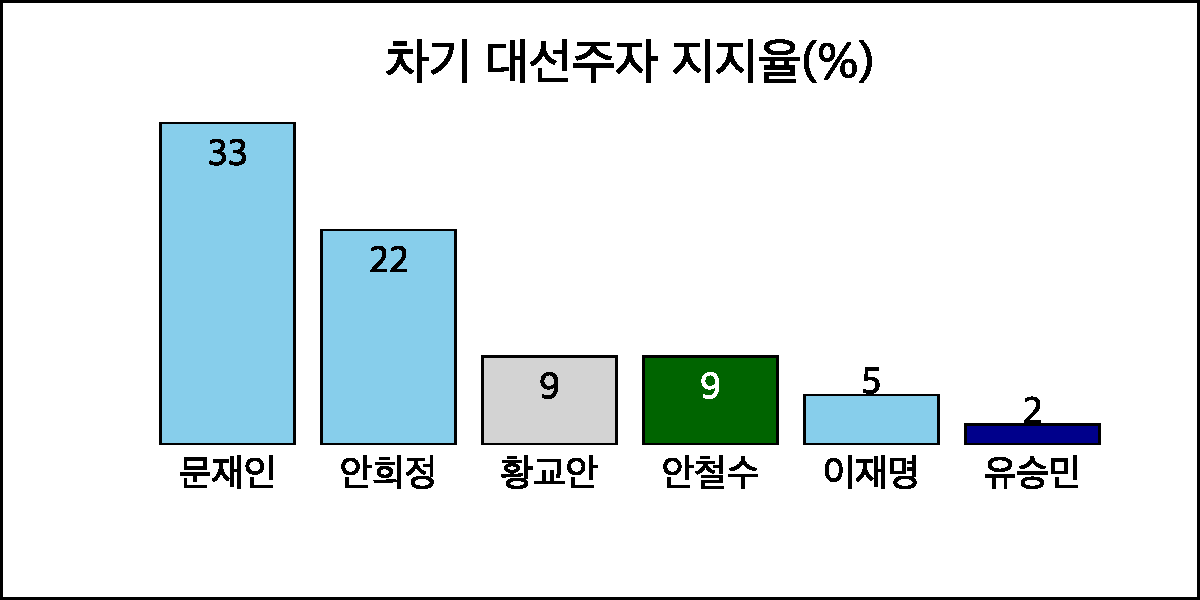
\includegraphics{poll_JTBC_1702_pdf_files/figure-latex/unnamed-chunk-3-1.pdf}

\begin{Shaded}
\begin{Highlighting}[]
\FunctionTok{dev.copy}\NormalTok{(png, }\StringTok{"../pics/jtbc1702.png"}\NormalTok{, }\AttributeTok{width =} \DecValTok{640}\NormalTok{, }\AttributeTok{height =} \DecValTok{320}\NormalTok{)}
\end{Highlighting}
\end{Shaded}

\begin{verbatim}
## quartz_off_screen 
##                 3
\end{verbatim}

\begin{Shaded}
\begin{Highlighting}[]
\FunctionTok{dev.off}\NormalTok{()}
\end{Highlighting}
\end{Shaded}

\begin{verbatim}
## cairo_pdf 
##         2
\end{verbatim}

\subsection{ggplot}\label{ggplot}

\begin{Shaded}
\begin{Highlighting}[]
\FunctionTok{library}\NormalTok{(ggplot2)}
\NormalTok{candidates }\OtherTok{\textless{}{-}} \FunctionTok{factor}\NormalTok{(candidates, }\AttributeTok{levels =}\NormalTok{ candidates)}
\NormalTok{rates\_df }\OtherTok{\textless{}{-}} \FunctionTok{data.frame}\NormalTok{(candidates, }
\NormalTok{                       candidates\_party, }
\NormalTok{                       candidates\_colour,}
\NormalTok{                       rates)}
\NormalTok{g0 }\OtherTok{\textless{}{-}} \FunctionTok{ggplot}\NormalTok{(}\AttributeTok{data =}\NormalTok{ rates\_df, }
             \AttributeTok{mapping =} \FunctionTok{aes}\NormalTok{(}\AttributeTok{x =}\NormalTok{ candidates, }
                           \AttributeTok{y =}\NormalTok{ rates))}
\NormalTok{(g1 }\OtherTok{\textless{}{-}}\NormalTok{ g0 }\SpecialCharTok{+}
  \FunctionTok{geom\_bar}\NormalTok{(}\AttributeTok{stat =} \StringTok{"identity"}\NormalTok{))}
\end{Highlighting}
\end{Shaded}

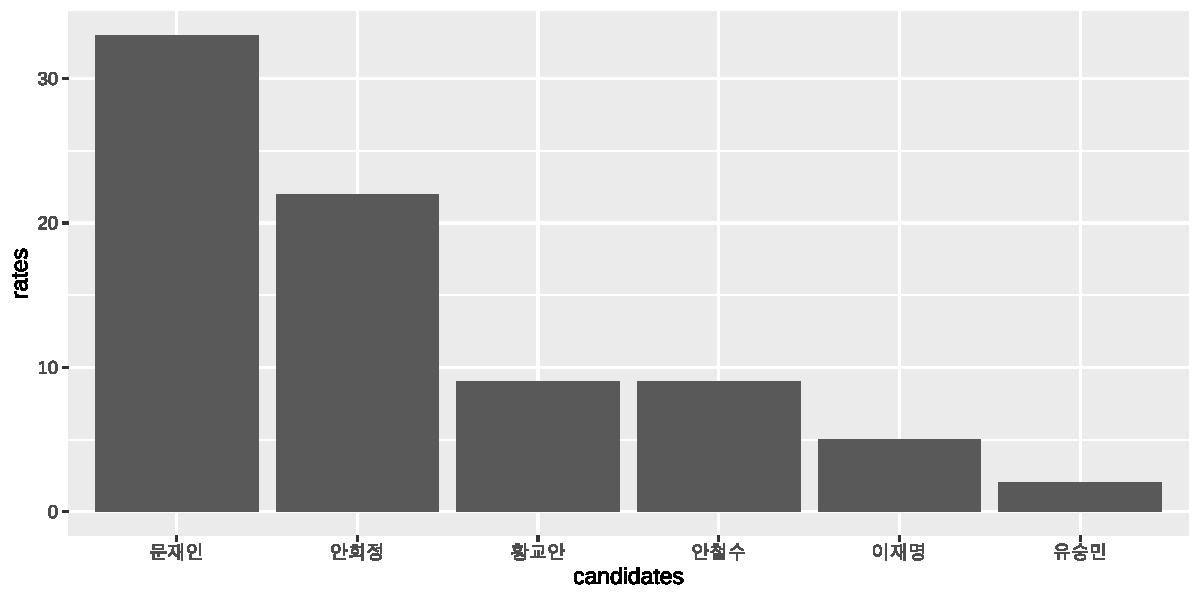
\includegraphics{poll_JTBC_1702_pdf_files/figure-latex/ggplot-1.pdf}

\begin{Shaded}
\begin{Highlighting}[]
\NormalTok{(g2 }\OtherTok{\textless{}{-}}\NormalTok{ g0 }\SpecialCharTok{+}
  \FunctionTok{geom\_bar}\NormalTok{(}\AttributeTok{stat =} \StringTok{"identity"}\NormalTok{, }
           \AttributeTok{fill =}\NormalTok{ candidates\_colour))}
\end{Highlighting}
\end{Shaded}

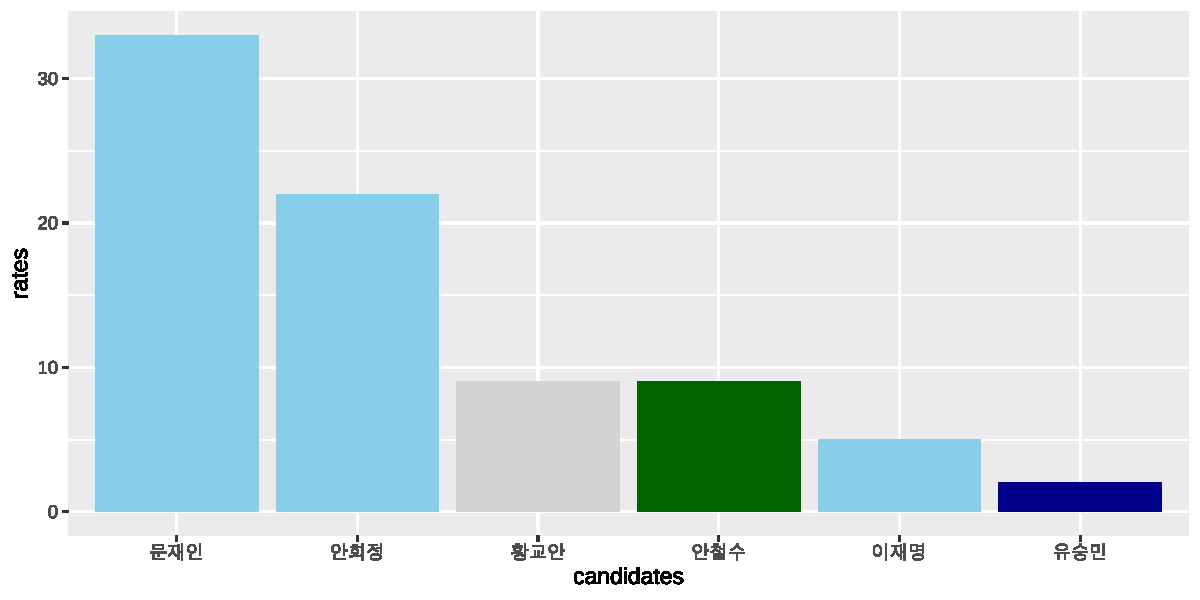
\includegraphics{poll_JTBC_1702_pdf_files/figure-latex/unnamed-chunk-4-1.pdf}

\begin{Shaded}
\begin{Highlighting}[]
\NormalTok{(g3 }\OtherTok{\textless{}{-}}\NormalTok{ g2 }\SpecialCharTok{+}
    \FunctionTok{theme\_bw}\NormalTok{(}\AttributeTok{base\_family =} \StringTok{"Apple"}\NormalTok{))}
\end{Highlighting}
\end{Shaded}

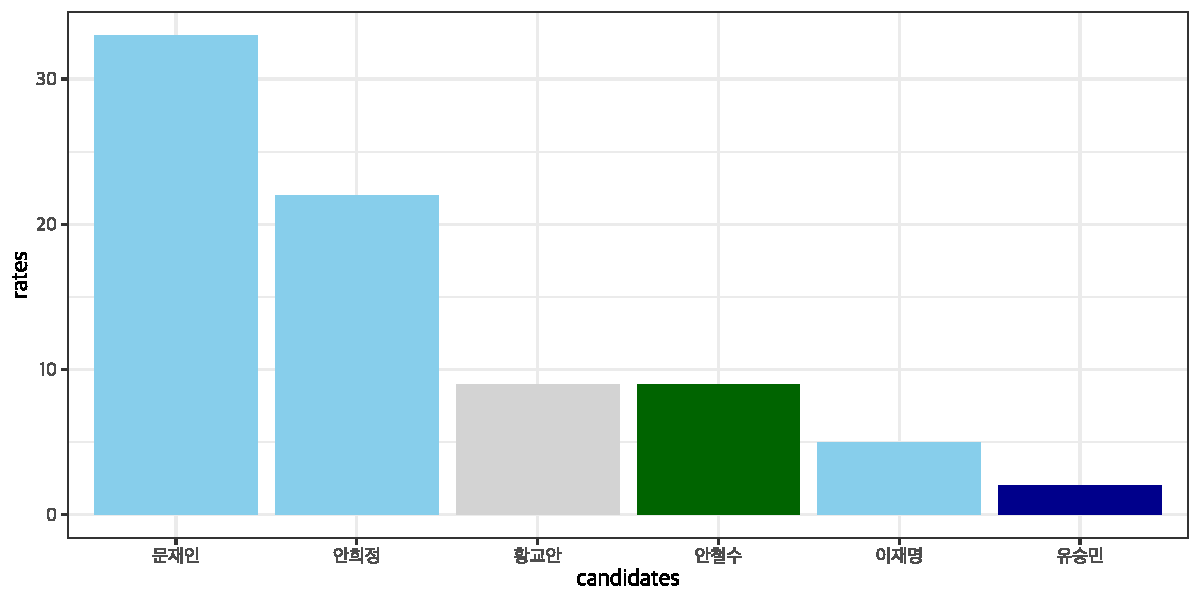
\includegraphics{poll_JTBC_1702_pdf_files/figure-latex/unnamed-chunk-4-2.pdf}

\begin{Shaded}
\begin{Highlighting}[]
\NormalTok{(g4 }\OtherTok{\textless{}{-}}\NormalTok{ g3 }\SpecialCharTok{+}
  \FunctionTok{geom\_text}\NormalTok{(}\AttributeTok{mapping =} \FunctionTok{aes}\NormalTok{(}\AttributeTok{x =}\NormalTok{ candidates, }
                          \AttributeTok{y =}\NormalTok{ rates }\SpecialCharTok{+} \FunctionTok{c}\NormalTok{(}\FunctionTok{rep}\NormalTok{(}\SpecialCharTok{{-}}\DecValTok{3}\NormalTok{, }\DecValTok{4}\NormalTok{), }\FunctionTok{rep}\NormalTok{(}\DecValTok{2}\NormalTok{, }\DecValTok{2}\NormalTok{)), }
                          \AttributeTok{label =}\NormalTok{ rates), }
            \AttributeTok{colour =} \FunctionTok{c}\NormalTok{(}\FunctionTok{rep}\NormalTok{(}\StringTok{"black"}\NormalTok{, }\DecValTok{3}\NormalTok{), }\StringTok{"white"}\NormalTok{, }\FunctionTok{rep}\NormalTok{(}\StringTok{"black"}\NormalTok{, }\DecValTok{2}\NormalTok{)),}
            \AttributeTok{size =} \DecValTok{6}\NormalTok{))}
\end{Highlighting}
\end{Shaded}

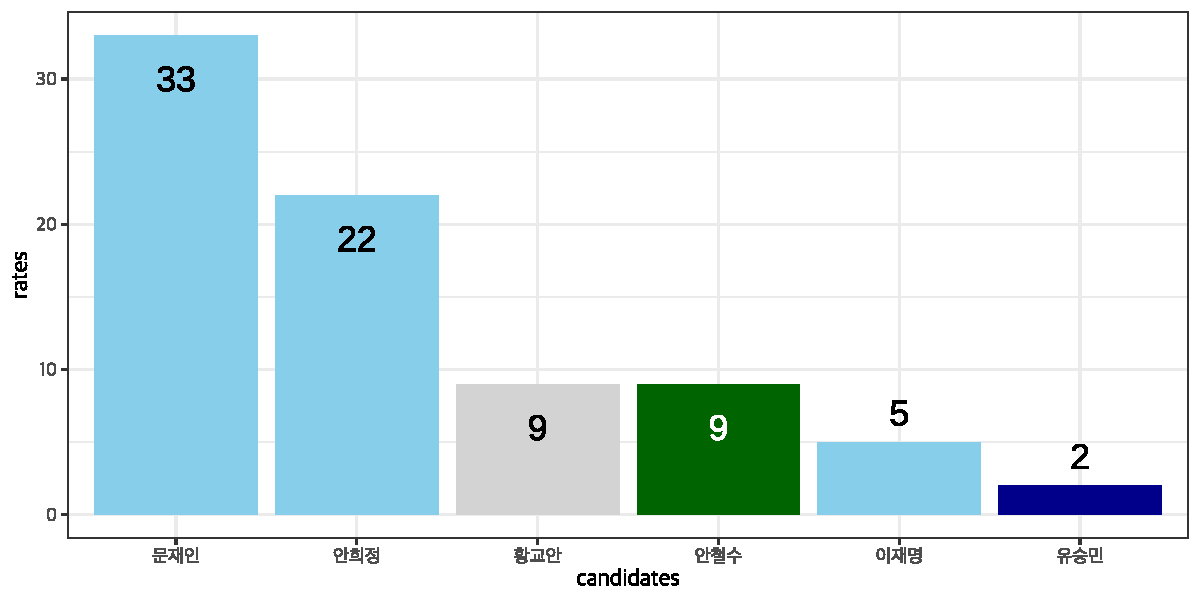
\includegraphics{poll_JTBC_1702_pdf_files/figure-latex/unnamed-chunk-4-3.pdf}

\begin{Shaded}
\begin{Highlighting}[]
\NormalTok{(g5 }\OtherTok{\textless{}{-}}\NormalTok{ g4 }\SpecialCharTok{+}
  \FunctionTok{labs}\NormalTok{(}\AttributeTok{title =}\NormalTok{ main\_title))}
\end{Highlighting}
\end{Shaded}

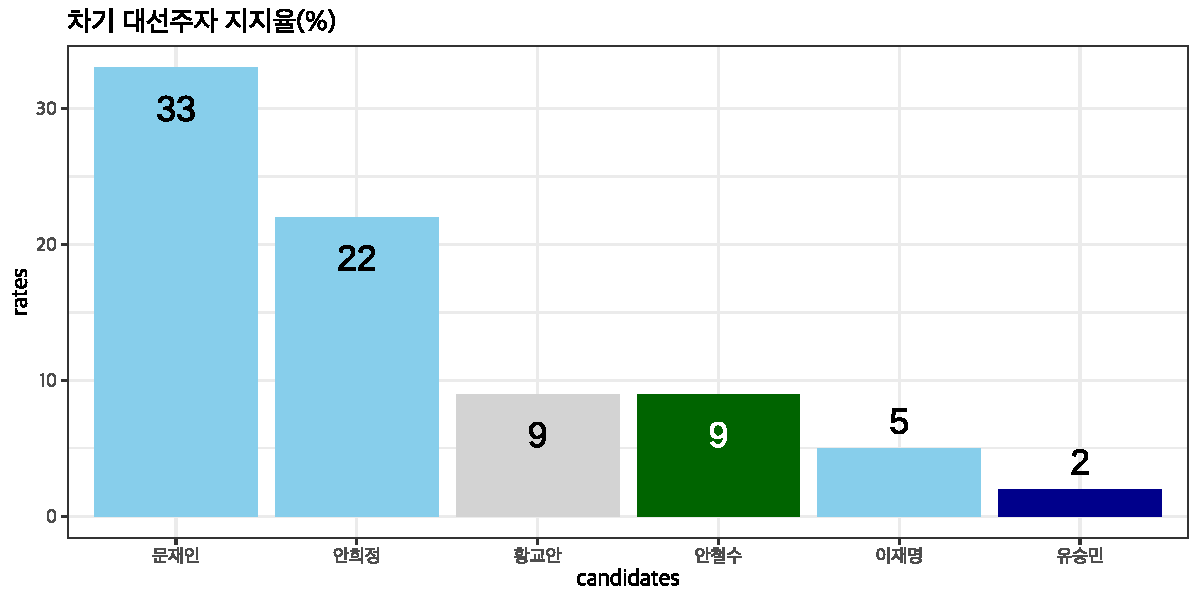
\includegraphics{poll_JTBC_1702_pdf_files/figure-latex/unnamed-chunk-4-4.pdf}

\begin{Shaded}
\begin{Highlighting}[]
\NormalTok{(g6 }\OtherTok{\textless{}{-}}\NormalTok{ g5 }\SpecialCharTok{+}
   \FunctionTok{theme}\NormalTok{(}\AttributeTok{plot.title =} \FunctionTok{element\_text}\NormalTok{(}\AttributeTok{family =} \StringTok{"Apple"}\NormalTok{,    }
                                  \AttributeTok{size =} \DecValTok{15}\NormalTok{, }
                                  \AttributeTok{hjust =} \FloatTok{0.5}\NormalTok{)))}
\end{Highlighting}
\end{Shaded}

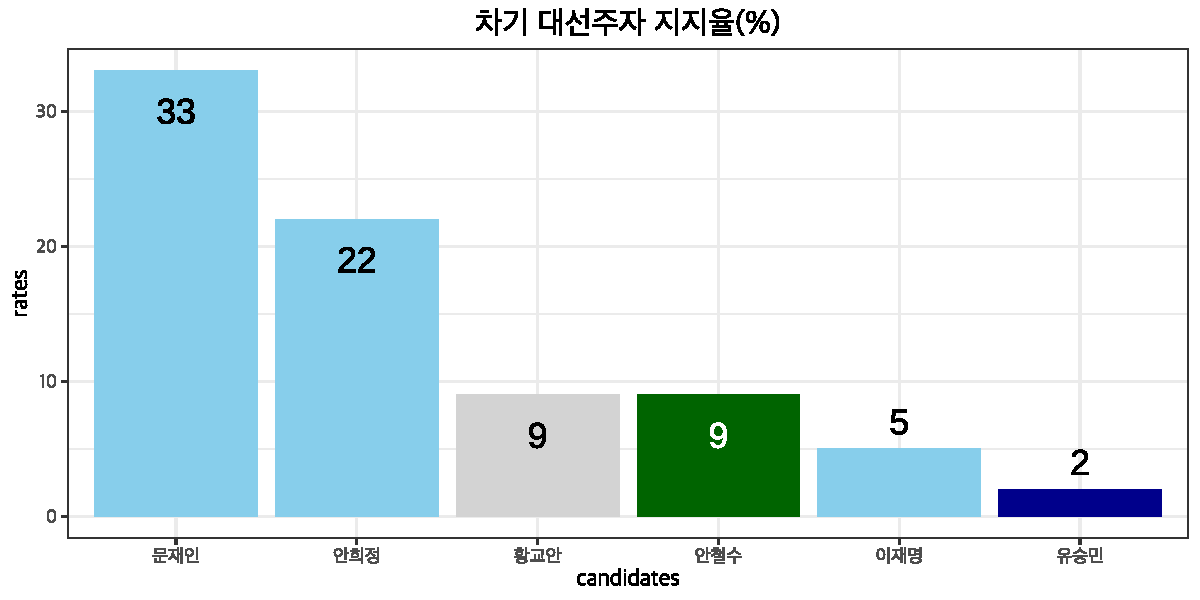
\includegraphics{poll_JTBC_1702_pdf_files/figure-latex/unnamed-chunk-5-1.pdf}

\begin{Shaded}
\begin{Highlighting}[]
\NormalTok{(g7 }\OtherTok{\textless{}{-}}\NormalTok{ g6 }\SpecialCharTok{+}
  \FunctionTok{scale\_y\_continuous}\NormalTok{(}\AttributeTok{breaks =}\NormalTok{ rates, }\AttributeTok{labels =}\NormalTok{ rates))}
\end{Highlighting}
\end{Shaded}

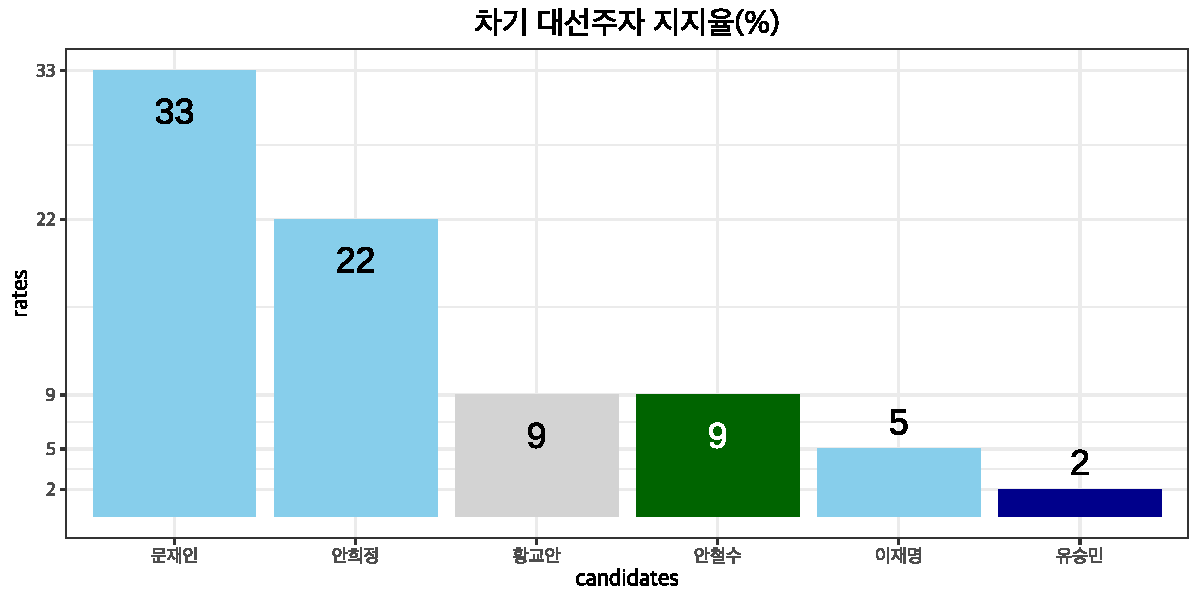
\includegraphics{poll_JTBC_1702_pdf_files/figure-latex/unnamed-chunk-5-2.pdf}

\begin{Shaded}
\begin{Highlighting}[]
\NormalTok{(g8 }\OtherTok{\textless{}{-}}\NormalTok{ g7 }\SpecialCharTok{+}
  \FunctionTok{theme}\NormalTok{(}\AttributeTok{panel.border =} \FunctionTok{element\_blank}\NormalTok{(),}
        \AttributeTok{axis.title.x =} \FunctionTok{element\_blank}\NormalTok{(),}
        \AttributeTok{axis.title.y =} \FunctionTok{element\_blank}\NormalTok{(),}
        \AttributeTok{axis.text.x =} \FunctionTok{element\_blank}\NormalTok{(),}
        \AttributeTok{axis.ticks =} \FunctionTok{element\_blank}\NormalTok{(), }
        \AttributeTok{axis.text.y =} \FunctionTok{element\_blank}\NormalTok{()))}
\end{Highlighting}
\end{Shaded}

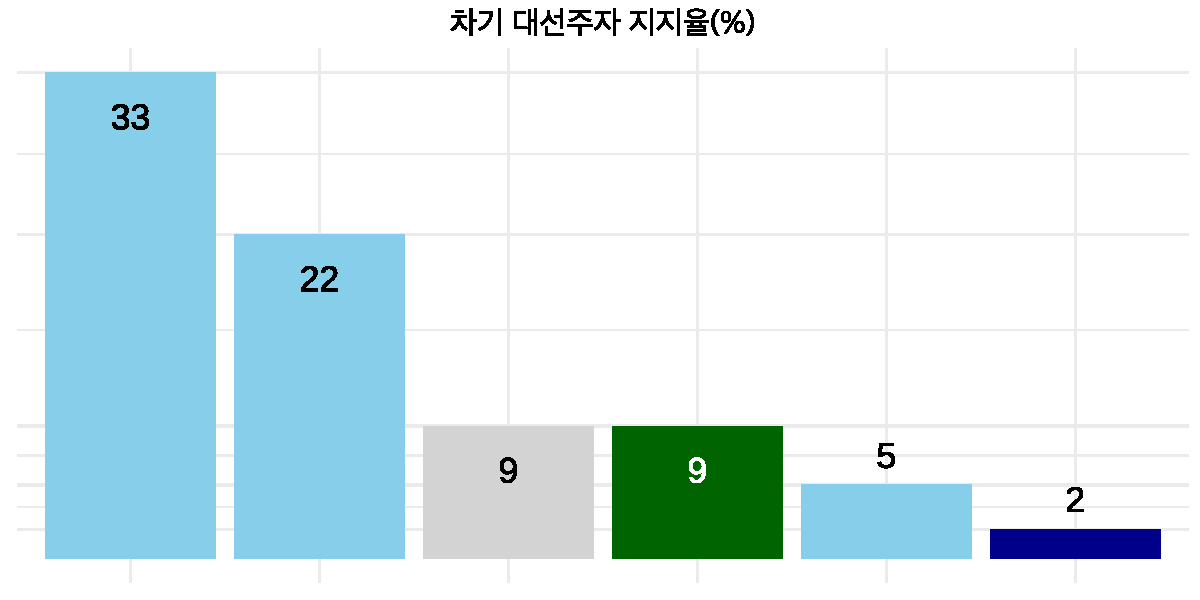
\includegraphics{poll_JTBC_1702_pdf_files/figure-latex/unnamed-chunk-6-1.pdf}

\begin{Shaded}
\begin{Highlighting}[]
\NormalTok{(g9 }\OtherTok{\textless{}{-}}\NormalTok{ g8 }\SpecialCharTok{+}
    \FunctionTok{geom\_text}\NormalTok{(}\AttributeTok{mapping =} \FunctionTok{aes}\NormalTok{(}\AttributeTok{x =}\NormalTok{ candidates,}
                            \AttributeTok{y =} \SpecialCharTok{{-}}\DecValTok{1}\NormalTok{,}
                            \AttributeTok{label =}\NormalTok{ candidates),}
              \AttributeTok{size =} \DecValTok{5}\NormalTok{,}
              \AttributeTok{family =} \StringTok{"Apple"}\NormalTok{))}
\end{Highlighting}
\end{Shaded}

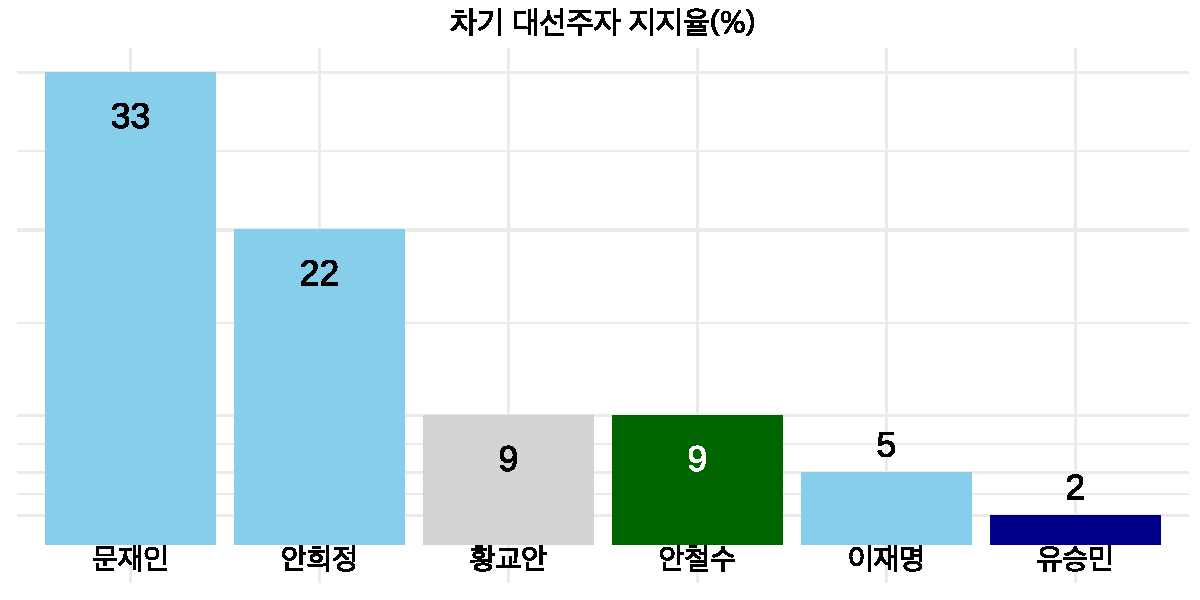
\includegraphics{poll_JTBC_1702_pdf_files/figure-latex/unnamed-chunk-7-1.pdf}

\begin{Shaded}
\begin{Highlighting}[]
\NormalTok{(g10 }\OtherTok{\textless{}{-}}\NormalTok{ g9 }\SpecialCharTok{+}
    \FunctionTok{ggtitle}\NormalTok{(}\StringTok{""}\NormalTok{) }\SpecialCharTok{+}
    \FunctionTok{annotate}\NormalTok{(}\StringTok{"text"}\NormalTok{, }
             \AttributeTok{x =} \FunctionTok{mean}\NormalTok{(b1), }
             \AttributeTok{y =} \ConstantTok{Inf}\NormalTok{, }
             \AttributeTok{label =}\NormalTok{ main\_title, }
             \AttributeTok{vjust =} \FloatTok{1.5}\NormalTok{, }
             \AttributeTok{size =} \DecValTok{6}\NormalTok{,}
             \AttributeTok{family =} \StringTok{"Apple"}\NormalTok{))}
\end{Highlighting}
\end{Shaded}

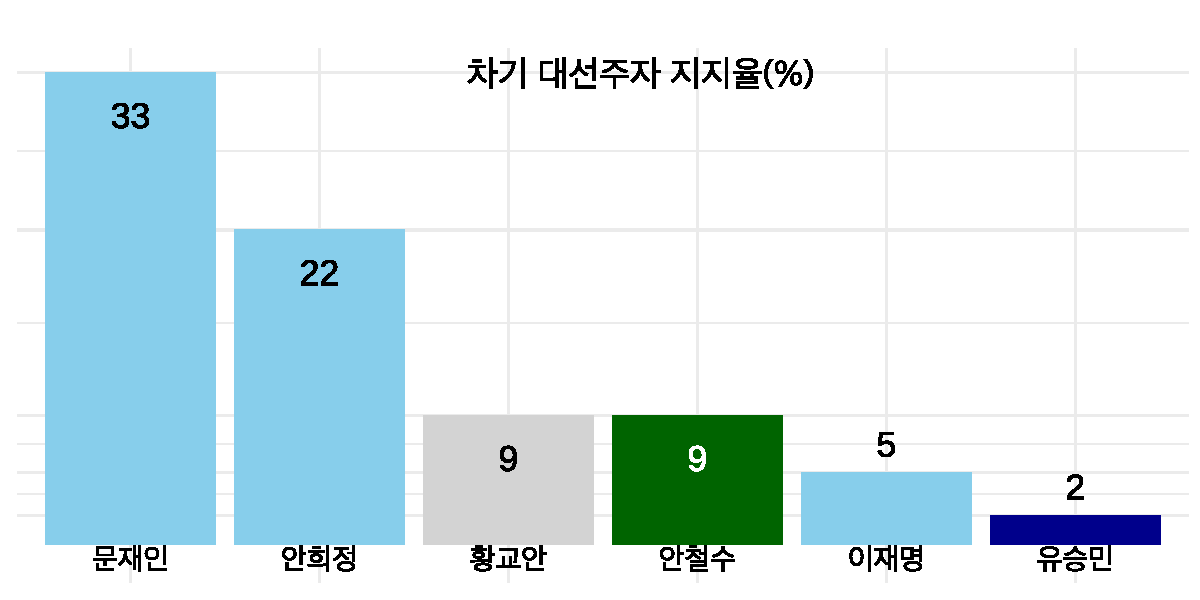
\includegraphics{poll_JTBC_1702_pdf_files/figure-latex/unnamed-chunk-8-1.pdf}

\begin{Shaded}
\begin{Highlighting}[]
\FunctionTok{library}\NormalTok{(gridExtra)}
\NormalTok{g\_all }\OtherTok{\textless{}{-}} \FunctionTok{grid.arrange}\NormalTok{(g1, g2, g3, g4, g5, g6, g7, g8, g9, g10, }\AttributeTok{nrow =} \DecValTok{5}\NormalTok{)}
\end{Highlighting}
\end{Shaded}

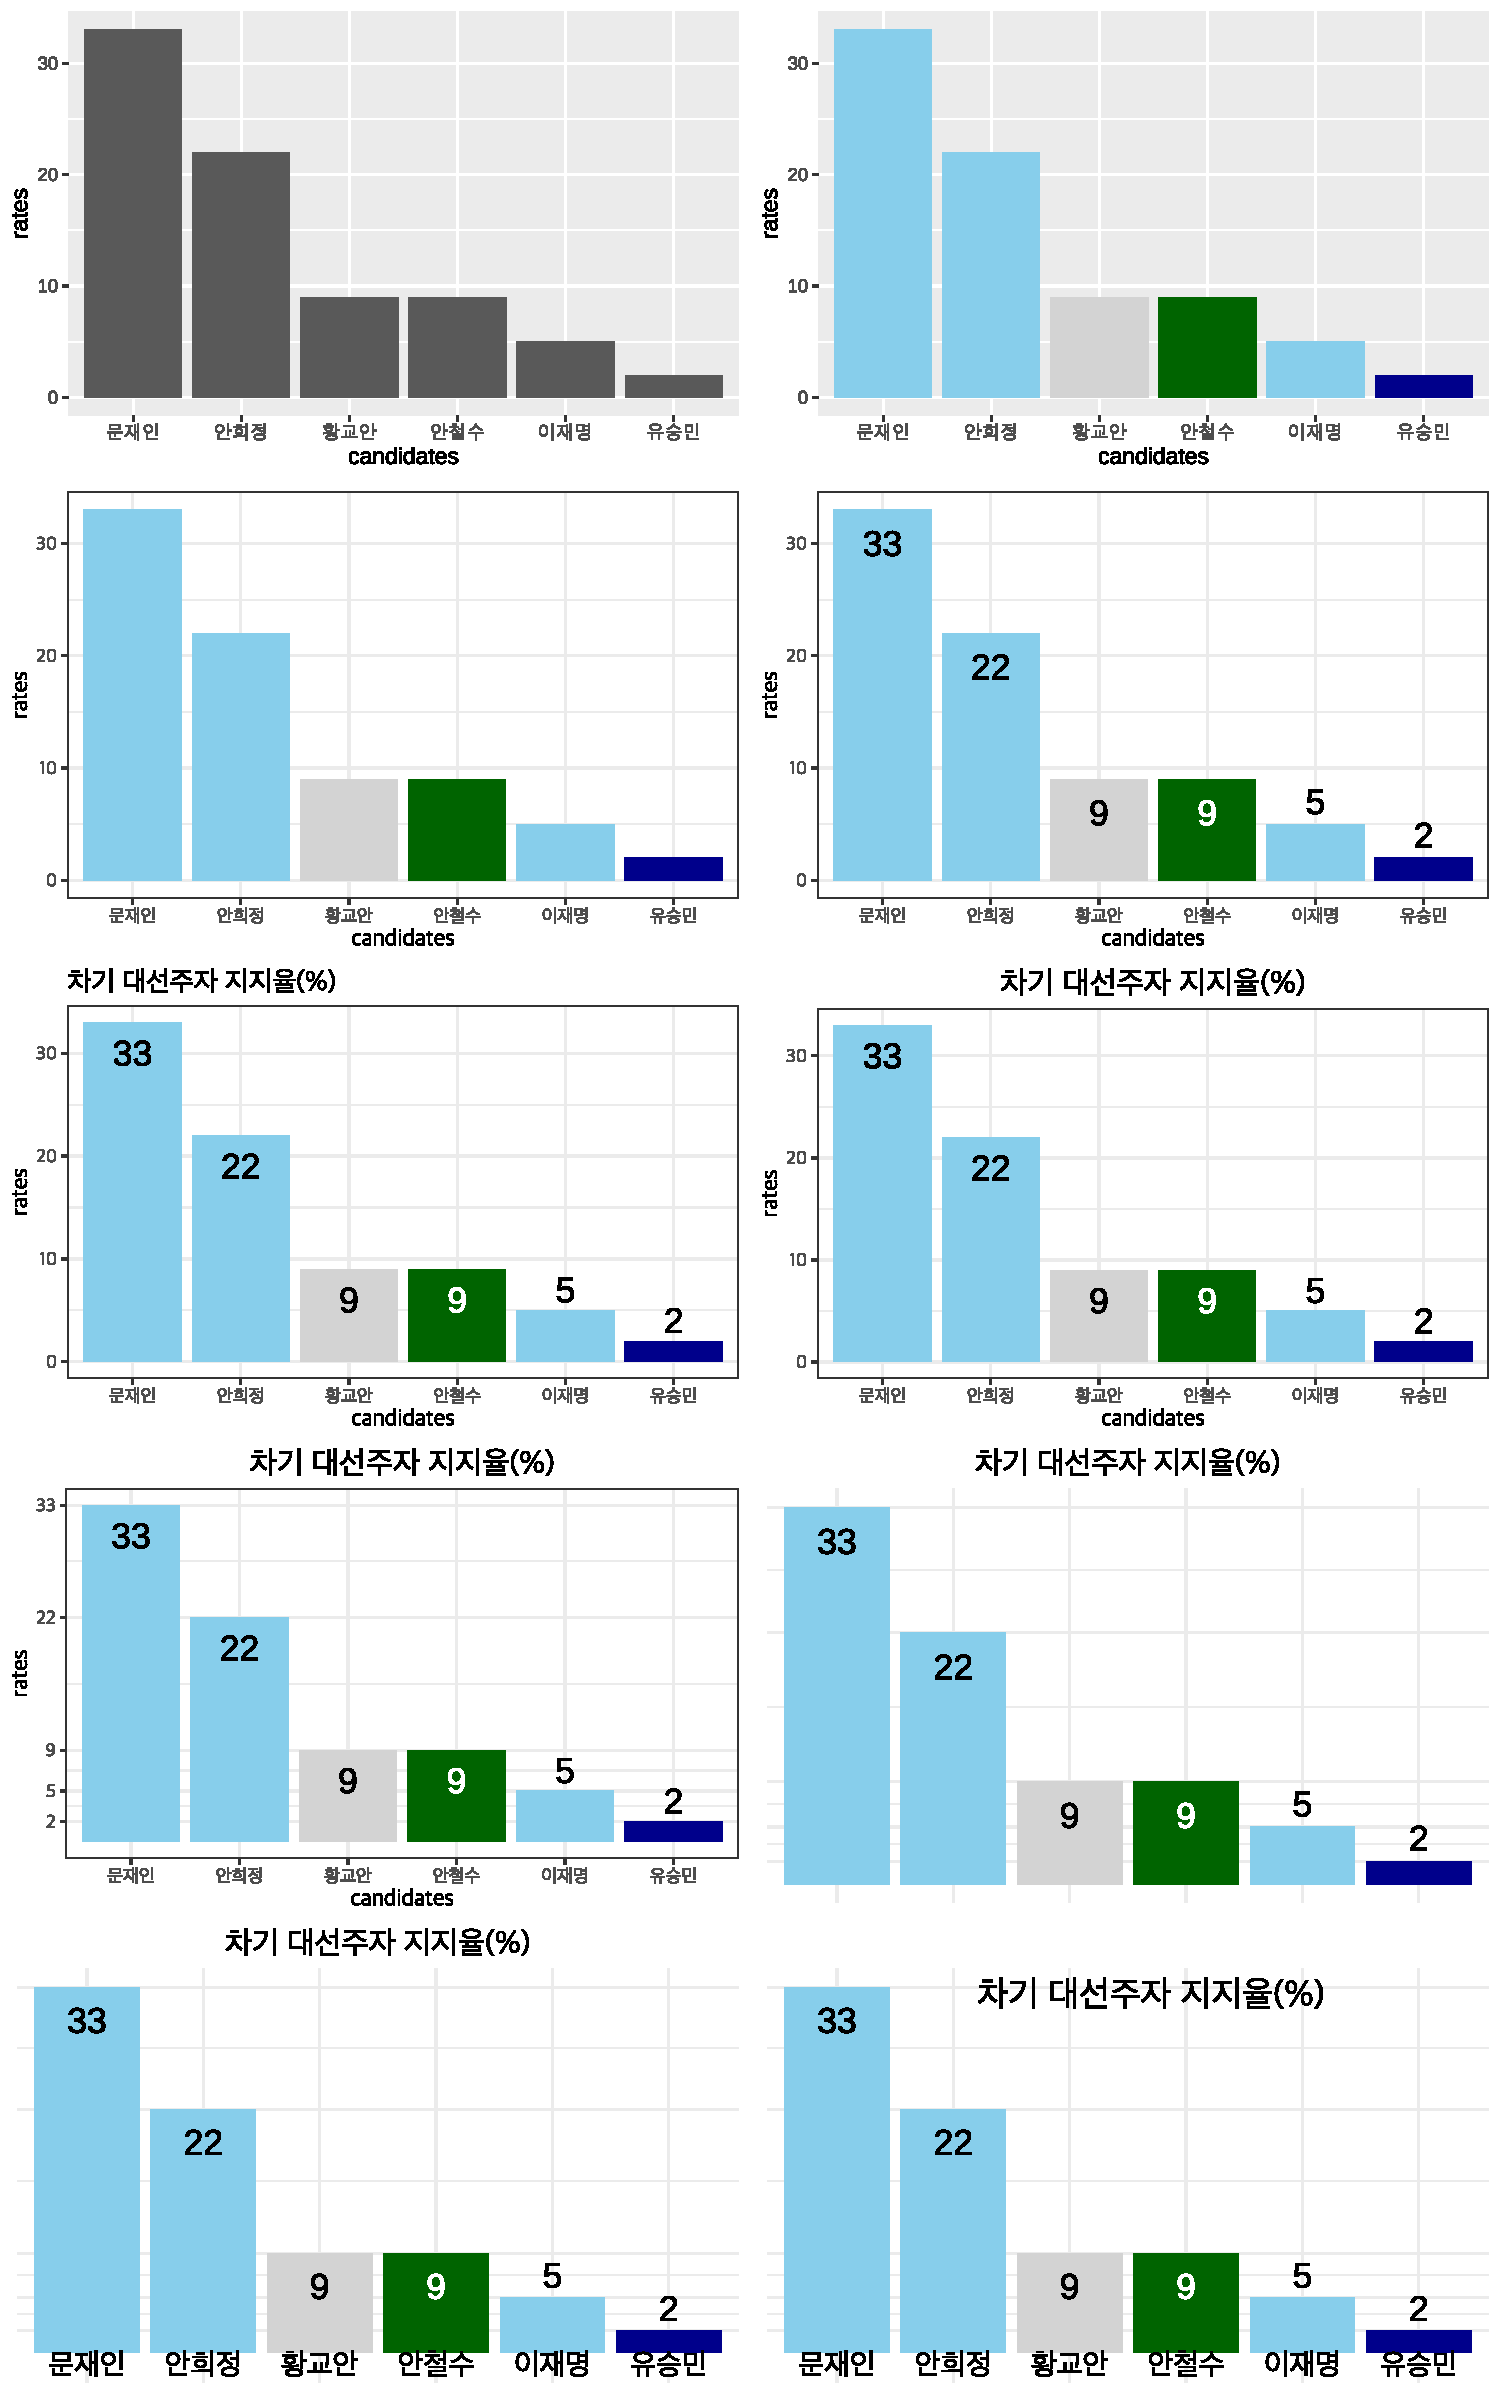
\includegraphics{poll_JTBC_1702_pdf_files/figure-latex/unnamed-chunk-9-1.pdf}

\begin{Shaded}
\begin{Highlighting}[]
\FunctionTok{ggsave}\NormalTok{(g10, }\AttributeTok{file =} \StringTok{"../pics/poll\_JTBC\_1702.png"}\NormalTok{, }\AttributeTok{width =} \DecValTok{8}\NormalTok{, }\AttributeTok{height =} \DecValTok{4}\NormalTok{)}
\FunctionTok{ggsave}\NormalTok{(g\_all, }\AttributeTok{file =} \StringTok{"../pics/poll\_JTBC\_1702\_plots.png"}\NormalTok{, }\AttributeTok{width =} \DecValTok{10}\NormalTok{, }\AttributeTok{height =} \DecValTok{16}\NormalTok{)}
\end{Highlighting}
\end{Shaded}

\subsection{Comments}\label{comments}

막대그래프를 이용한 눈속임에 대하여 느낀 바를 간단히 기술하세요.

\end{document}
